\documentclass[border=2pt]{standalone}
\usepackage{tikz}
\usepackage{amsmath}
\usepackage{mathtools}
\usepackage{adjustbox}
\usetikzlibrary{patterns}
\usetikzlibrary{calc} \usetikzlibrary{positioning} \usetikzlibrary{shapes,arrows} \usetikzlibrary{plotmarks}
\usetikzlibrary{positioning,decorations.pathreplacing}
\tikzset{
litria/.style={
  draw,shape border uses incircle,
  isosceles triangle,shape border rotate=90,yshift=-0.3cm,xshift=0.1cm},
ritria/.style={
  draw,shape border uses incircle,
  isosceles triangle,shape border rotate=90,yshift=-0.3cm,xshift=-0.1cm}
}

\begin{document}

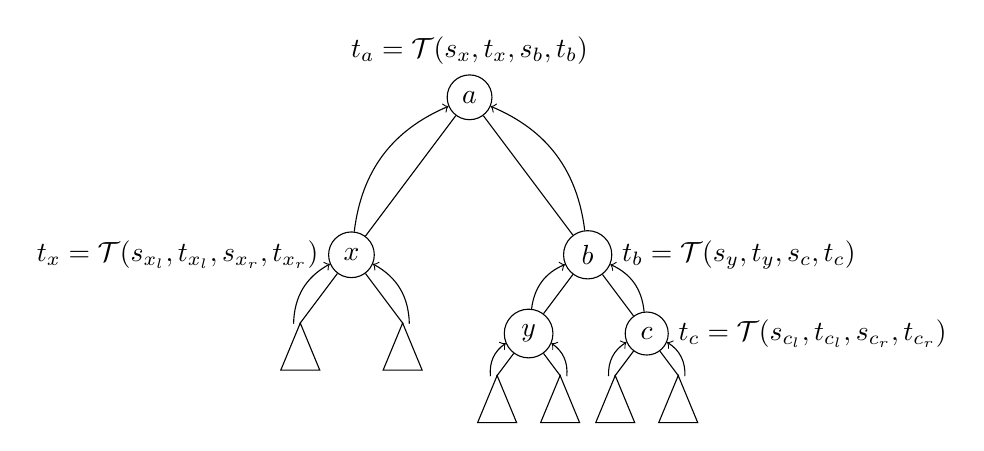
\begin{tikzpicture}[level/.style={sibling distance=30mm/#1, level distance=20mm/#1},baseline=(Atid.base)]
\node[circle,draw](Atid){$a$}
    child { node[circle,draw](Alsub){$x$}
        child {
          node(xlsub)[]{}
          {node[litria]{}}
        }
        child {
          node(xrsub)[]{}
          {node[ritria]{}}
        }
    }
    child { node[circle,draw](Btid){$b$}
      child { node[circle,draw](Blsub){$y$}
        child {
          node(ylsub)[]{}
          {node[litria]{}}
        }
        child {
          node(yrsub)[]{}
          {node[ritria]{}}
        }
      }
      child { node[circle,draw](Brsub){$c$}
        child {
          node(clsub)[]{}
          {node[litria]{}}
        }
        child {
          node(crsub)[]{}
          {node[ritria]{}}
        }
      }
  };

\path[solid,->](Alsub)edge [bend left=30]  (Atid);
\path[solid,->](xlsub)edge [bend left=30]  (Alsub);
\path[solid,->](xrsub)edge [bend right=30]  (Alsub);
\path[solid,->](clsub)edge [bend left=30]  (Brsub);
\path[solid,->](crsub)edge [bend right=30]  (Brsub);
\path[solid,->](ylsub)edge [bend left=30]  (Blsub);
\path[solid,->](yrsub)edge [bend right=30]  (Blsub);
\path[solid,->](Btid)edge [bend right=30]  (Atid);
\path[solid,->](Blsub)edge [bend left=30]  (Btid);
\path[solid,->](Brsub)edge [bend right=30]  (Btid);

\node[above=0cm of Atid]{$t_{a}={\cal T}(s_{x}, t_{x}, s_{b}, t_{b})$};
\node[left=0cm of Alsub]{$t_{x}={\cal T}(s_{x_l}, t_{x_l}, s_{x_r}, t_{x_r})$};
\node[right=0cm of Btid]{$t_{b}={\cal T}(s_{y}, t_{y}, s_{c}, t_{c})$};
\node[right=0cm of Brsub]{$t_{c}={\cal T}(s_{c_l}, t_{c_l}, s_{c_r}, t_{c_r})$};

\end{tikzpicture}

\end{document}